\chapter {The Mastermodule}
\label{Mastermodule}

The Mastermodule is a generic framework for the implementation of 
OpenCms modules. 
It consist of generic classes (especially the generic Content Definition class \\
{\class com.opencms.defaults.master.CmsMasterContent}) and database tables that are
designed to suit the needs of common modules.

In the past, when implementing your own modules the design and access to the database tables
used by a module had to be designed and implemented new for every module.
From now on this functionality is already implemented in the mastermodule and can be used
in your own modules.

The database tables used by the mastermodule contain fields for common information like the title,
the creation date, the date of last modification etc. and also fields for 
text, numbers, dates and binary data that can be freely used by your modules.

The mastermodule also provides functionality like the integration of Content Definition entries in the
projectmechanism and the use of channels (they work similar to folders) to organize Content Definition entries.
An entry can be associated with one or more channels.
These channels can be used to filter the data and show only entries which belong to a certain channel.

Beside this the MasterContentDefinition provides constructors to create new empty objects or to read an 
entry from the database. And also the {\meth write()} and {\meth delete()} methods that write
changes to the database or delete an entry are already implemented. In the old way of writing Content Definitions
these methods had to be written new for every module.

Another feature that is already included is the access-control for Content Definition entries: each
entry belongs to a user and group and also has its own access rights like other resources in the vfs.
If someone has not the appropriate rights he will not be able to edit a Content Definition entry.

Here is a short summary of the improvements coming with the Mastermodule:

\begin{itemize}
\item generic database design with fields for text, numbers, dates and binary data
\item access to database (constructors, {\meth write()}, {\meth delete()}) already implemented
\item entries are fully integrated in the projectmechanism
\item manages access-rights for the entries
\item entries can be organized through channels
\item simplified backoffice implementation
\end{itemize}


Also the implementation of backoffice functionality has been simplified. 
A new class {\class com.opencms.defaults.A\_CmsChannelBackoffice} provides support for the
managing of channels and media files (binary data) in the backoffice. The template
extended\_backoffice in the folder /system/workplace/templates/ can be used for creating
backoffice edit templates. It includes a template for upload of media files (binary data, 
accessible in the Content Definition via the method {\meth getMedia()})
and selection of channels in the backoffice. To use the backoffice list view with 
integration of the projectmechanism you have to override the method {\meth isExtendedList()}
to return true in your backoffice class. 
There are also new methods added in the backoffice class that return special urls:

\begin{itemize}
\item[-] getHistoryUrl() returns the url for the history view 
\item[-] getPublishUrl() returns the url for publishing
\item[-] getUndeleteUrl() returns the url for undeletion
\end{itemize}

To write a Content Definition class it must be inherited from the 
{\class CmsMasterContent} class and implement the following methods:

\begin{itemize}
\item[-] {\meth getSubId()} (returns a unique SUB\_ID to identify entries of a module)
\item[-] {\meth get()} and {\name set()} methods (to access the module data)
\item[-] filtermethods for backoffice filters 
\item[-] {\meth getFilterMethods()} (returns the filtermethods used in the backoffice)
\item[-] {\meth getFieldNames()} (returns the column headings of the backoffice list) 
\item[-] {\meth publishProject()} (called when the data is published)
\item[-] {\meth moduleParameterWasUpdated()} (event-method that reads module parameters)
\end{itemize}

The access to the database is encapsulated in a class {\name CmsDbAccess} that resides in a subpackage
of the module. You can write multiple {\name CmsDbAccess} classes for support of different databases.
The type of the database can then be controlled by a moduleparameter (e.g. {\name dbType}) and an
object of the appropriate {\name CmsDbAccess} class can be created.

The following sections will describe the purpose of the different methods
and show some examples how to implement them. The methods {\meth getFilterMethods()} and {\meth getFieldNames()} 
have already been introduced in chapter ~\ref{ideacontentdefinition} 
(page \pageref{ideacontentdefinition}) about Content Definitions and can be looked up there.

The method {\name getSubId()} is declared as an abstract method in the class 
{\class CmsMasterContent} and should return a unique id for the module. Because 
all data of modules using the Mastermodule is inserted in one database table it
is necessary to have a unique identifier for entries of a module.:

\begin{verbatim}
/** unique SUB-ID for this Content Definition */
 protected static final int C_SUB_ID = 1;

/**
 * Returns the sub-id of this Content Definition.
 */
 public int getSubId() {
     return C_SUB_ID;
 }
\end{verbatim}

The {\name get()} and {\name set()} methods provide access to the module data. 
The object m\_dataSet of type {\class CmsMasterDataSet} is defined in the {\class CmsMasterContent}
class and contains the member variables that actually hold the data:

\begin{verbatim}
 /**
  * Returns the name
  */
 public String getName() {
      return m_dataSet.m_dataSmall[0];  }

 /**
  * Sets the name
  */
 public void setName(String newName) {
     m_dataSet.m_dataSmall[0] = newName;
 }
\end{verbatim}

As you can see the methods access an array {\name m\_dataSmall} which is contained
in the {\name m\_dataSet} object. The Mastermodule provides String variables in the 
arrays {\name m\_dataSmall}, {\name m\_dataMedium} and {\name m\_dataBig}
which are mapped to database text fields of different size 
and also the arrays {\name m\_dataDate} and {\name m\_dataInt} for date and int fields.
Currently the Mastermodule tables includes these free usable fields:

\begin{itemize}
\item 40 fields DATA\_SMALL\_0  ... DATA\_SMALL\_39 for short Strings
\item 10 fields DATA\_MEDIUM\_0 ... DATA\_MEDIUM\_9 for longer Strings
\item 10 fields DATA\_BIG\_0    ... DATA\_BIG\_9 for extra long Strings
\item 10 fields DATA\_INT\_0    ... DATA\_INT\_9 for integer values
\item 5  fields DATA\_DATE\_0   ... DATA\_DATE\_4 for date values
\end{itemize}

The main decision to make when implementing the {\meth get()} and {\meth set()}
methods is what information should be stored in which database field 
and under what name should it be accessible. 

Filtermethods in the Content Definition class delegate the database access
to the {\class CmsDbAccess} class of the module. The filtermethod must have a parameter
of type {\class CmsObject} and can have additional parameters to be used in the database query.
The method has to return a Vector of Content Definition objects:

\begin{verbatim}
 /**
  * Filter method.
  * @param cms - the CmsObject to get access to the cms ressources.
  * @return a Vector of Content Definition.
  */
 public static Vector filterAll(CmsObject cms) throws CmsException {
     return ((CmsDbAccess)getDbAccessObject(C_SUB_ID)).filterAll
             (cms, CmsContentDefinition.class, C_SUB_ID);
 }
\end{verbatim}


The actual database query will be executed in a filtermethod in the {\class CmsDbAccess} class:

\begin{verbatim}
public Vector filterAll(CmsObject cms, Class contentDefinitionClass, int subId)
{
	try {
		// get a connection from the connection pool
		Connection con = getConnection(cms);
   
		// prepare the statement filter_all
		PreparedStatement stmnt = sqlPrepare(cms, con, "filter_all");
   
		// set the value for the sub_id in the statement
		stmnt.setInt(1, subId);
   
		// execute the query and get the result
		ResultSet res = stmnt.executeQuery();
   
		// build a Vector of Content Definition objects from the result
		// boolean parameter viewonly set to true to return only entries 
		// which are allowed to be viewed by the current user (v-right)
		return createVectorOfCd(res, contentDefinitionClass, cms, true);
	} catch(SQLException exc) {
		exc.printStackTrace(System.err);
		throw new CmsException("Error accessing database.",
			CmsException.C_SQL_ERROR, exc);
	} finally {
		sqlClose(con, stmnt, res);
	}   
}
\end{verbatim}

The filtermethod first gets a connection of the connection pool and then uses a prepared
statement to execute the query.
The SQL-statements are stored in a property file query.properties which is located in the folder of
the {\class CmsDbAccess} class:

\begin{verbatim}
filter_all : \
    select ${colum_names_master} \
    from $CMS_MODULE_MASTER \
    where sub_id = ? \
    order by title;
\end{verbatim}

The query uses two variables to specify the columns and the name of the table. 
By using a variable for the column names you can be sure that you always use the correct names.
Because OpenCms uses different tables for the online and offline data, the variable for the tablename
will be replaced with CMS\_MODULE\_ONLINE\_MASTER or \\
CMS\_MODULE\_MASTER depending on the actual project your are in.
If you would decide to use explicit table names you had to use different statements for the online and offline tables.

The mechanism of the database access in the mastermodule can be seen in figure~\ref{databasemaster}.

\begin{figure}[!hbt]
\begin{center}
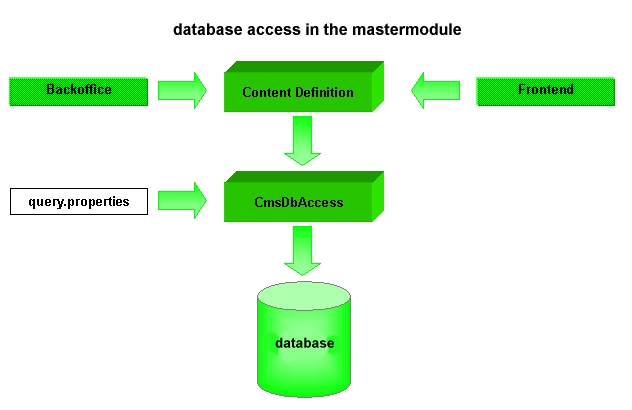
\includegraphics[clip,width=\sgw]{pics/modules/masterclasses}
\end{center}
\caption[database access in the mastermodule]
    {database access in the mastermodule}
\label{databasemaster}
\end{figure}

The method {\meth publishProject()} must be implemented to publish the module data. You can take
this example implementation and only have to replace the name of the Content Definition class:

\begin{verbatim}
public static void publishProject(CmsObject cms, Boolean enableHistory,
            Integer projectId, Integer versionId, Long publishingDate,
            Vector changedRessources, Vector changedModuleData) 
            throws CmsException {

        // publish the ressources for this module
        CmsMasterContent.publishProject(
            cms, 
            enableHistory.booleanValue(),
            projectId.intValue(), 
            versionId.intValue(),
            publishingDate.longValue(), 
            C_SUB_ID, 
            YourContentDefinition.class.getName(),
            changedRessources, 
            changedModuleData
        );
    }
\end{verbatim}

To make sure that this method gets called when the project is published you also have to 
provide the name of the Content Definition class in the {\name registry.xml} file of 
OpenCms inside the section for your module:

\begin{verbatim}
<modules>
  <module>
    <name>module.package</name>
      ...
      <publishclass>
        <name>module.package.YourContentDefinition</name>
      </publishclass>
      ...
   </module>
</modules>
\end{verbatim}

The method {\meth moduleParameterWasUpdated()} is used to read the module parameters from the 
OpenCms {\name registry.xml} file. The method is automatically invoked on the eventhandling class 
of the module (this should be your Content Definition class)
when the parameters are changed via the module administration of OpenCms. The mastermodule uses 
several parameters to provide the database urls for online, offline and backup tables and the type of the database:

\begin{verbatim}
/**
 * Reads the module parameters from the registry.
 * Automatically invoked when the parameters are changed
 * in the module administration.
 * @param cms - CmsObject to access system resources.
 */
 public static void moduleParameterWasUpdated(CmsObject cms) 
         throws CmsException {
     // read all poolnames from the module parameters
     String connect = OpenCms.getRegistry().getModuleParameterString(
         "module.package", "onlinePool", "jdbc:opencmspool:mysqlonline");
     String connectOffline = OpenCms.getRegistry().getModuleParameterString(
         "module.package", "offlinePool", "jdbc:opencmspool:mysql");
     String connectBackup = OpenCms.getRegistry().getModuleParameterString(
         "module.package", "backupPool", "jdbc:opencmspool:mysqlbackup");
     // read the dbtype from the module properties
     String dbType = OpenCms.getRegistry().getModuleParameterString(
         "module.package", "dbType", "genericsql");
     // read the root channel from the module properties
     String rootChannel = OpenCms.getRegistry().getModuleParameterString(
         "module.package", "rootChannel", "/");

     if("genericsql".equalsIgnoreCase(dbType)){
         CmsDbAccess dbAccess = 
		     new CmsDbAccess(connectOffline, connect, connectBackup);
         CmsMasterContent.registerDbAccessObject(C_SUB_ID, dbAccess);
         dbAccess.setRootChannel(rootChannel);
     } else {
         throw new CmsException("No database selected");
     }
}
\end{verbatim}

The method reads the parameters {\name onlinePool}, {\name offlinePool} and {\name backupPool}
that define the jdbc urls for access to the online, offline and backup tables of the module.
The third String parameter in the method call to {\meth getModuleParameterString()} is a default
value that will be returned by the method if the parameter is not specified in the {\name registry.xml} 
file. If you omit this parameter the method will return null if the parameter cannot be found.
The parameter {\name dbType} is used to control which database will be used. Depending on this
parameter the appropriate CmsDbAccess object will be created with the urls for the online, offline 
and backup tables. Another module parameter is the {\name rootChannel} parameter. It is used to
define a parent channel for all channels accessible for this module. For example if the root channel
is set to /news/ all subchannels of /news/ will be available in the backoffice to put a news entry
in it. This way you have a seperation of channels of different modules. The value of the {\name rootChannel}
must be set in the {\name CmsDbAccess} object. 
If you don't set it, it will be set to the default value, the root folder ("/"). So if you don't need channels
in your module you can simply forget about this parameter.
 
%%% Local Variables:
%%% mode: latex
%%% TeX-master: "OpenCmsDoc"
%%% End:
